\section{Class imbalance}
\label{sec:imbalance}

With 23.9\% of positives, a model can look accurate while missing most of the
\pos{} people; Section~\ref{sec:eda} listed the metrics we report instead of
accuracy alone. Here we compare three ways of handling the imbalance, from the
least to the most invasive, on the three untuned models
(Table~\ref{tab:imbalance}).
\begin{itemize}
  \item \textbf{No remedy}: the model as it is, with the default threshold 0.5.
  \item \textbf{Class weights}: \code{class\_weight="balanced"} gives both
  classes the same total weight, so each \pos{} person weighs
  $N_{\text{neg}}/N_{\text{pos}} \approx 3.2$ times a \negc{} person. The
  weights are computed inside each fit, on the training folds only. The model
  is retrained, so its probabilities change.
  \item \textbf{Threshold tuning}: the model without weights, but the cut-off
  0.5 is replaced by the threshold that maximizes F1 on the out-of-fold
  probabilities (grid from 0.05 to 0.95, step 0.01). The model is not
  retrained: only the decisions change. We maximize F1 because the dataset comes
  with no business cost for each type of error, and F1 assumes that a false
  positive and a false negative cost about the same.
\end{itemize}
We did not use SMOTE. It creates synthetic people by interpolating between
neighbours, which has no meaning for our seven categorical features: there is
nothing halfway between two occupations or two countries.

\begin{table}[H]
\centering
\caption{Imbalance remedies on the untuned models (5-fold out-of-fold
predictions on the development set). AP and log-loss judge the probabilities;
precision, recall and F1 judge the decisions at the given threshold.}
\label{tab:imbalance}
\small
\setlength{\tabcolsep}{4pt}
\begin{tabular}{llrrrrrr}
\toprule
Model & Remedy & AP & Log-loss & Precision & Recall & F1 & Threshold \\
\midrule
Log. regression     & None         & 0.784 & 0.309 & 0.747 & 0.613 & 0.673 & 0.50 \\
                    & Class weights & 0.783 & 0.379 & 0.576 & 0.852 & 0.687 & 0.50 \\
                    & Threshold     & 0.784 & 0.309 & 0.659 & 0.745 & \textbf{0.699} & 0.36 \\
\midrule
Random forest       & None          & 0.750 & 0.446 & 0.711 & 0.624 & 0.665 & 0.50 \\
                    & Class weights & 0.724 & 0.510 & 0.629 & 0.743 & \textbf{0.681} & 0.50 \\
                    & Threshold     & 0.750 & 0.446 & 0.622 & 0.750 & 0.680 & 0.33 \\
\midrule
LightGBM            & None          & 0.831 & 0.275 & 0.779 & 0.653 & 0.711 & 0.50 \\
                    & Class weights & 0.830 & 0.332 & 0.605 & 0.867 & 0.713 & 0.50 \\
                    & Threshold     & 0.831 & 0.275 & 0.708 & 0.756 & \textbf{0.731} & 0.38 \\
\bottomrule
\end{tabular}
\end{table}

\paragraph{What we learn.} At the default threshold, the models find only 61\%
to 65\% of the \pos{} people. Both remedies trade precision for recall, but in
different ways.
\begin{itemize}
  \item \textbf{Class weights} raise recall strongly (from 0.613 to 0.852 for
  the logistic regression) at a high cost in precision (from 0.747 to 0.576),
  for a small F1 gain. They do not improve the ranking: AP is unchanged for the
  logistic regression and LightGBM, and drops from 0.750 to 0.724 for the
  random forest. They also worsen the log-loss of all three models (from 0.275
  to 0.332 for LightGBM): weighting pushes the probabilities up, so they no
  longer match the observed frequencies.
  \item \textbf{Threshold tuning} gives the best F1 for the logistic regression
  (0.699) and LightGBM (0.731), and ties with class weights for the random
  forest, without retraining and without touching the probabilities. The
  chosen thresholds (0.33 to 0.38) are well below 0.5, as expected with a
  minority class. This F1 is slightly optimistic, since the threshold is
  chosen and scored on the same out-of-fold probabilities; with one parameter
  and 39{,}032 rows the bias is small, and the honest value comes from the
  test set.
\end{itemize}

\begin{figure}[H]
\centering
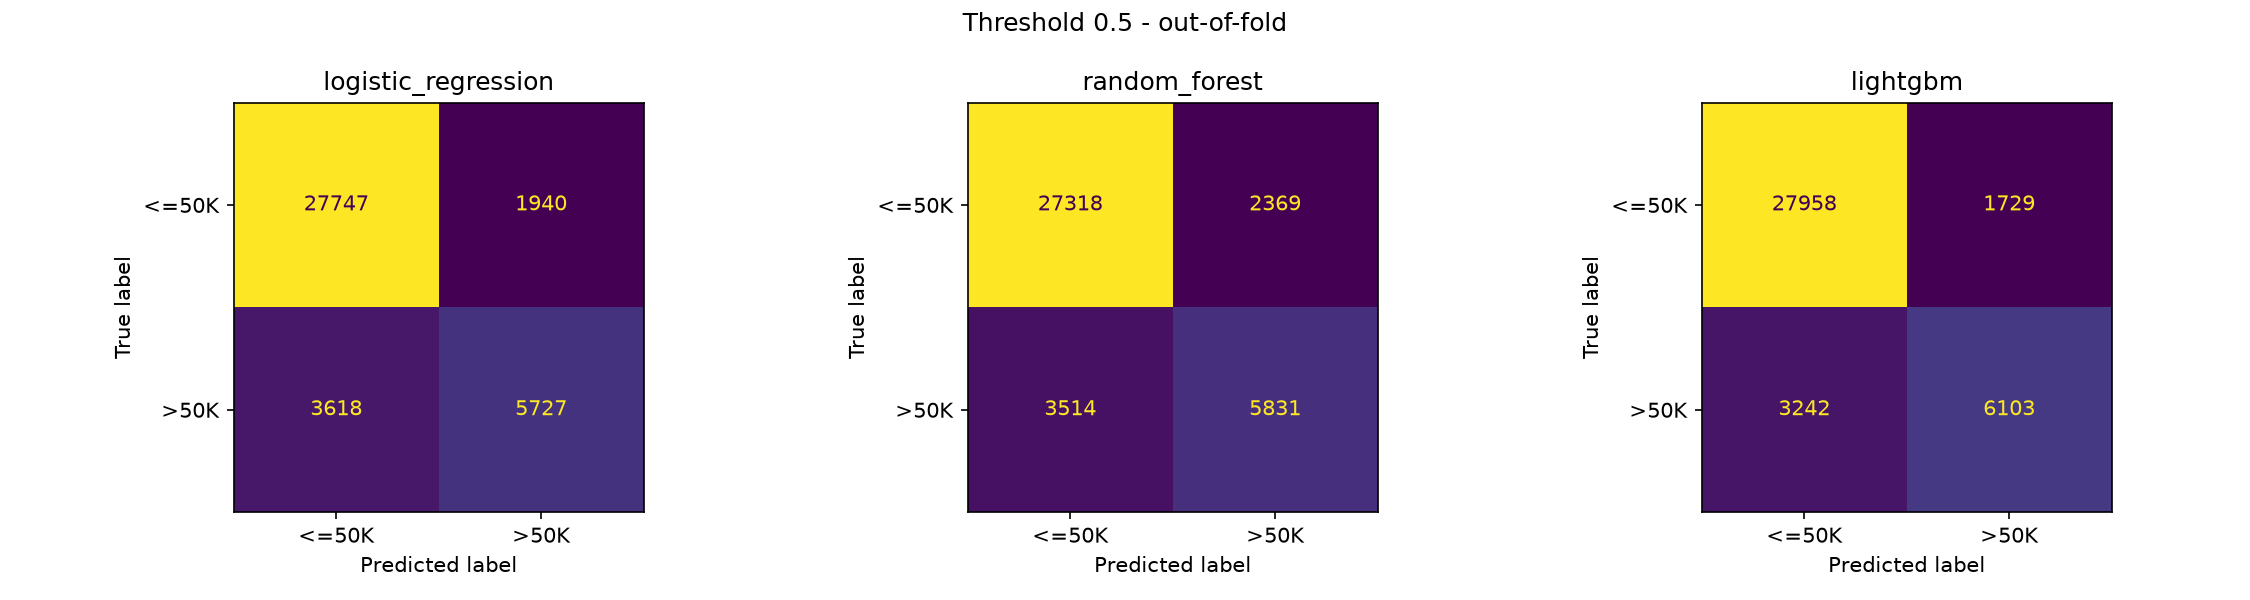
\includegraphics[width=0.9\textwidth]{baseline_confusion_default.png}\\[4pt]
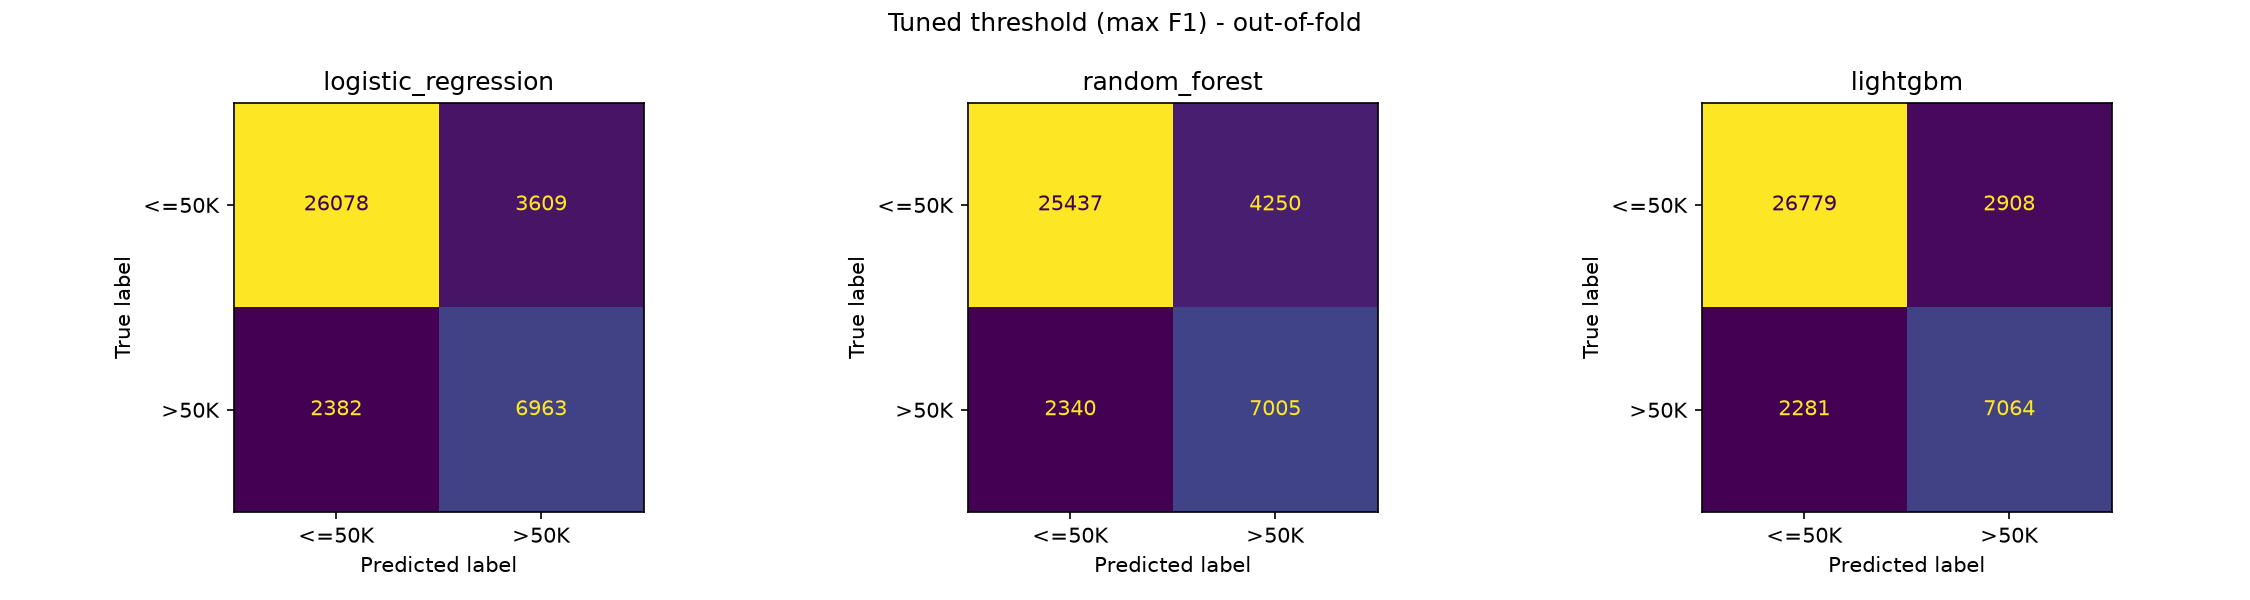
\includegraphics[width=0.9\textwidth]{baseline_confusion_tuned.png}
\caption{Out-of-fold confusion matrices of the untuned models, at the threshold
0.5 (top) and at the threshold that maximizes F1 (bottom).}
\label{fig:confusion-baseline}
\end{figure}

\paragraph{Chosen remedy.} We keep both levers, each in its place. The class
weight becomes a hyperparameter that Optuna may use or not
(Section~\ref{sec:tuning}): \code{class\_weight} $\in$ \{None, balanced\} for
the logistic regression and the random forest, and \code{scale\_pos\_weight}
$\in [1, 3.18]$ for LightGBM. Then the decision threshold is chosen on the
out-of-fold probabilities of each tuned model and frozen before the test set
is used. Section~\ref{sec:calibration} comes back to the price of class
weighting on the probabilities.
